\chapter{Grundlagen}\label{kap:grundlagen}

%####################  CHAPTER 1: Grundlagen  #################

Im folgende Kapitel wird zunächst auf die Grundlegenden Techniken
 des Machine Learings, insbesondere auf die für die Bilderkennung 
verwendeten Convolutional Neural Networks eingegangen.

Anschließend wird es um die verwendete Hardware, den Neural 
Compute Stick 2 un seine Anwendungen gehen.


%------------------- SECTION: Machine Learning ------------------

\section{Machine Learning}\label{sec:ml}

Beim Machine Lerining, welches ein Teilgebiet der Computerwissenschafen
ist, geht es um Algorithmen, die Zusammenhänge in großen Datenmengen 
erkennen sollen, ohne expliziet darauf programmiert worden zu sein.

Eine Form davon ist das \textit{Supervised Learning}, bei der das Programm 
neben den Input Daten auch die Zugehörigen Ausgaben erhällt und daraus 
dann die Regeln für Zusammenhänge herleiten soll.
Dadurch unterscheidet sich das Vorgehen wesentlich zur klassischen Programmierung,
bei bei der die Regeln vorab definiert werden.

\vspace{0.5cm}
\begin{figure}[htb]
    \centering
    \def\svgwidth{0.8\columnwidth}
    \footnotesize
    
\tikzset{
    decision/.style={
        diamond,
        draw,
        text width=4em,
        text badly centered,
        inner sep=-1pt,
        node distance=8em
    },
    block/.style={
        rectangle,
        draw,
        text width=6em,
        %minimum widhth=6em,
        minimum height=5em,
        text centered,
        node distance=20em
    },
    arrow/.style={
        draw,
        >=latex,
        ->
    },
    textfeld/.style={
        %draw,
        text centered,
        node distance=1.5em
    }
}


\begin{tikzpicture}

    
    \node (system) [block] {Klassisches\\Programm};
    \node (system2) [block, right of=system] {Machine Learning\\Programm};

    \node [textfeld, left=of system.162] (inputs) {Daten};
    \node [textfeld, left=of system.198] (regeln) {Regeln};
    \node [textfeld, right=of system] (output) {Ausgaben};

    \node [textfeld, left=of system2.162] (inputs2) {Daten};
    \node [textfeld, left=of system2.198] (output2) {Ausgaben};
    \node [textfeld, right=of system2] (regeln2) {Regeln};
    
    \draw[arrow] (inputs) -- (system.162);
    \draw[arrow] (regeln) -- (system.198);
    \draw[arrow] (system) -- (output);
    
    \draw[arrow] (inputs2) -- (system2.162);
    \draw[arrow] (output2) -- (system2.198);
    \draw[arrow] (system2) -- (regeln2);
    

\end{tikzpicture}

\end{figure}
\vspace{0.5cm}

Das herleiten der Regeln erfolgt beim Machine Learning dabei in einem 
iterativen Prozess, welcher als Training bezeichnet wird.
Dabei soll eine math. Funktion, welche die Zusammenhänge beschreibt 
numerisch angenähert werden. Ist der Zusammenhang linear, spricht man 
von einer Regrassion, handelt es sich um Kategorische, liegt 
ein Klassifizierung problem vor.
\\
Weitere Formen neben dem \textit{Supervised Learning} sind das 
\textit{Unsupervised Learning}, bei der das Programm keine Labels 
erhällt, sondern diese durch Clustering Verfahren selber finden 
soll, oder das \textit{Reinfocement Learning}, bei dem das Programm 
mit der Umwelt interagieren soll.
\\
Da hier jedoch ausschließlich mit dem Supervised Learing gearbeitet
wurde, werden diese Techniken nicht näher erläutert.


%------------------- SECTION: Neuronale Netze -------------------

\subsection{Künstliche Neuronale Netze} \label{subsec:nn}

Für komplexe Input Daten, wie beispielsweise Bilder, bei denen 
die einzelnen Pixelwerte als Inputs und der Inhalt des Bildes als 
Output dienen, werden in der Regel künstliche Neuronale Netze verwendet.
Diese sind eine Form des Machine Learings und bestehen aus einer 
vielzahl an miteinander verbundener Neuronen. Durch unterschiedlich 
starke Gewichtungen der einzelnen Verbindungen, auch Gewichte genannt, 
können für unterschiedliche Input Daten die entsprechenden Outputs 
gefunden werden.

\begin{figure}[htb]
    \centering
    \label{fig:nn}
    \def\svgwidth{0.5\columnwidth}
    \footnotesize
    \begin{neuralnetwork}[height=1]
    \newcommand{\nodetextclear}[2]{}
    \newcommand{\nodetexth}[2]{$h_#2$}
    \newcommand{\nodetextx}[2]{$x_#2$}
    \newcommand{\nodetexty}[2]{$y_#2$}
    \inputlayer[count=3, bias=false, title=Input\\layer, text=\nodetextx]
    \hiddenlayer[count=4, bias=false, title=Hidden\\layer, text=\nodetexth] \linklayers
    \outputlayer[count=2, title=Output\\layer, text=\nodetexty] \linklayers
\end{neuralnetwork}
\end{figure}


Die richtige einstellung der Gewichte, welche zunächst zufällig initialisiert werden, 
erfolgt dabei im Trainingsprozess, welcher in \ref{fig:train} schematisch
 dargestellt ist und sich in die drei Schritte:
\begin{itemize}
    \item Feed Forward anhand aktueller Gewichte vorhersage aus den Inputs treffen
    \item Lossfuction Abweichung zu tatsächlichen werten bestimmen
    \item Backpropagation minimierung der Fhlerfunktion durch anpassung der Gewichte
\end{itemize}

\begin{figure}[htb]
    \centering
    \label{fig:train}
    \def\svgwidth{0.5\columnwidth}
    
\tikzstyle{process} = [rectangle, fill=blue!20, minimum width=2.5cm, minimum height=1cm, text centered, draw=black]
\tikzstyle{arrow} = [thick,->,>=stealth]

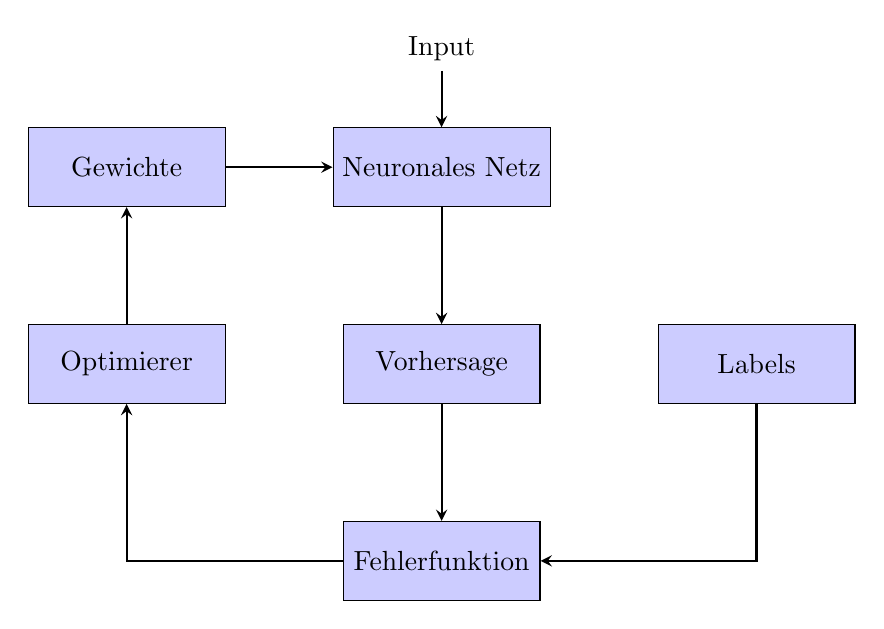
\begin{tikzpicture}[node distance=1.6cm]

  \begin{scope}[node distance=2.5cm]
    \node (nn)      [process]                   {Neuronales Netz};
    \node (pred)      [process, below of=nn]      {Vorhersage};
    \node (loss)      [process, below of=pred]      {Fehlerfunktion};
    
  \end{scope}
  
  \begin{scope}[node distance=4cm]
    \node (opt) [process, left of=pred]      {Optimierer};
    \node (weights)  [process, left of=nn] {Gewichte};
    \node (labels)   [process, right of=pred]  {Labels};
  \end{scope}

  \node (input) at (0,1.5) {Input};

  \draw[arrow] (input) -- (nn);

  \draw[arrow] (nn) -- (pred);
  \draw[arrow] (pred) -- (loss);

  \draw[arrow] (labels) |- (loss);
  \draw[arrow] (loss) -| (opt);

  \draw[arrow] (opt) -- (weights);
  \draw[arrow] (weights) -- (nn);
  
    
\end{tikzpicture}

    \caption{Trainingsablauf NN}
\end{figure}

Durch häufiges wiederholen dieser Schritte kann die Fehlerfunktion soweit minimiert werde, 
dass das Modell auch für neue Input Daten die richtigen Aussagen treffen kann.


\subsubsection{Vorwärts}
Im Vorwärtsdurchgang wird der Input durch alle Schichten hindurch 
gereicht, um in der letzten Schicht den gewünschten Output zu liefern.
Dabei erhält jedes Neuron wie in \ref{fig:neuron} dargestellt, die Ausgabewerte
aller Neuronen der vorherigen Schicht, summiert diese auf und übergibt den Wert
an eine Aktivierungsfunktion, die den Wert auf einen bestimmten Bereich skaliert.


\begin{figure}[h]
    \centering
    \label{fig:neuron}
    \begin{tikzpicture}[
    % define styles    
    init/.style={ 
         draw, 
         circle, 
         inner sep=2pt,
         font=\Huge,
         join = by -latex
    },
    squa_draw/.style={ 
        draw,
        font=\Large,
        join = by -latex
    },
    squa/.style={ 
        font=\Large,
        join = by -latex
    }
]
% Top chain x1 to w1
\begin{scope}[start chain=1]
    \node[on chain=1] at (0,1.5cm)  (x1) {$x_1$};
    \node[on chain=1,join=by o-latex] (w1) {$w_1$};
\end{scope}
% Middle chain x2 to output
\begin{scope}[start chain=2]
    \node[on chain=2] (x2) {$x_2$};
    \node[on chain=2,join=by o-latex] {$w_2$};
    \node[on chain=2,init] (sigma) {$\displaystyle\Sigma$};
    \node[on chain=2,squa_draw,label=below:{\parbox{2cm}{\centering Aktivierungs\\ Funktion}}]   {$\delta(z)$};
    \node[on chain=2,squa,label=below:Output,join=by -latex] {$y_{out}$};
\end{scope}
% Bottom chain x3 to w3
\begin{scope}[start chain=3]
    \node[on chain=3,label=below:Inputs] at (0,-1.5cm) 
    (x3) {$x_3$};
    \node[on chain=3,label=below:Gewichte,join=by o-latex]
    (w3) {$w_3$};
\end{scope}
% Bias
\node[label=above:\parbox{2cm}{\centering Bias \\ $b$}] at (sigma|-w1) (b) {};
% Arrows joining w1, w3 and b to sigma
\draw[-latex] (w1) -- (sigma);
\draw[-latex] (w3) -- (sigma);
\draw[o-latex] (b) -- (sigma);

\end{tikzpicture}

% von https://medium.com/momenton/typesetting-neural-network-diagrams-with-tex-4920b6b9fc19
    \caption{Einzelnes Perzeptron}
\end{figure}






Die Berechnung des Vorwärtsdurchgangs einer ges Schicht aus Neuronen
als Vektor $z$ dargestellt, erfolgt wie in \cite{goodfellowDeepLearning2016a}
beschrieben, über die Matrixmultiplikation des Vektors
$x$ der vorherigen Schicht mit der Gewichtsmatrix $W$.

\begin{equation}
    \label{eq:forward}
    z = W^{T}x+b
\end{equation}

und wird anschließend elementweise einer nichtlinearen Aktivierungsfunktion
$g(z)$ übergeben.\\
Für Hidden Schichten wird dabei üblicherweisse in \ref{eq:relu} dargestellte
\textit{ReLU} verwendet eine Funktion die negative Werte zu 0 setzt.

\begin{equation}
    \label{eq:relu}
    g(z) = max\{0,z\}
\end{equation}

Da die Ausgabe meist einen Wahrscheinlichkeites Wert zwischen 0 und 1 
haben soll wird für die letzte Schicht bei einer binären Klassifikation 
die \textit{Sigmoid} Funktion \ref{eq:sidmoid}

\begin{equation}
    \label{eq:sidmoid}
    g(z) = \frac{1}{1 + e^{-x}}
\end{equation}

verwendet und für kategorische Ausgaben die \textit{Softmax} \ref{eq:softmax}
Funktion.
\begin{equation}
    \label{eq:softmax}
    g(z) = \frac{e^{z}}{\sum e^{x}}
\end{equation}



\subsubsection{Fehlerfunktion}
Die Abweichung der Schätzung, welche an den Neuronen der letzen Schicht 
vorliegen, zu den tatsächlichen Werten, den Labels, wird mithilfe geeigneter 
Fehlerfunktion bestimmt. Für Ragression z.B. abs oder rms und für Kategorisch
häufig logarithmisch.

hier am beispiel einer binären klassifikation (erg 0 oder 1) mit log loss
 (crossentropy) dargestellt.

 \begin{equation}
    \label{eq:crossentropy}
    L = \hat{y}log(y) + (1 - \hat{y})log(1 - y)
\end{equation}

Durch den Logarithmus wird der Loss um so größer, je weiter die Schätzung $y$ vom 
tatsächlichen Wert $\hat{y}$ abweicht.
%hier plot


\subsubsection{Backpropagation}
Durch berechnung des Gradienten der Fehlerfunktion kann ermittelt 
werden in welche Richtung die Gewichte angepasst werden müssen, sodass sie sich 
im nächsten Durchgang minimiert.
Dafür wird die die Fehlerfunktion für jede Schicht partiell nach den 
Gewichten abgeleitet, was wie in gl. \ref{eq:backprop} dargestellt mithilfe der 
Kettenregel für die Aktivierungsfunktion geschieht.


\begin{equation}
    \label{eq:backprop}
    \frac{\partial L}{\partial w} = \frac{\partial L}{\partial z}\frac{\partial z}{\partial w}
\end{equation}
Damit werden die Gewichte dann nach Gleichung \ref{eq:update_wieghts} angepasst.
\begin{equation}
    \label{eq:update_wieghts}
    w  \leftarrow w - \eta \frac{\partial L}{\partial w}
\end{equation}

wobei die \textit{Leariningrate} $\eta$ die Schrittweite mit der die Anpassung vorgenommen
werden soll angibt.








%------------------- SUBSECTION: Validierung -------------------
\subsection{Validierung und Overfitting}\label{subsec:validation}

um überprüfen zu können ob ein Modell die Trainingsdaten tatsächlich generalisiert 
hat, dh auch für neue daten anwendbar ist, oder diese nur auswendig gelernt hat, 
wird häufig der Datensatz in einen Trainingsanteil und einen Testanteil aufgeteilt.

Mit dem Testdatensatz wird dann schon wärend des Trainings regelmäßig zwischen geprüft, 
veringert sich irgendwann nur noch der fehler der trainingsdaten, findet overfitting statt.

% \begin{figure}[htb]
%     \centering
%     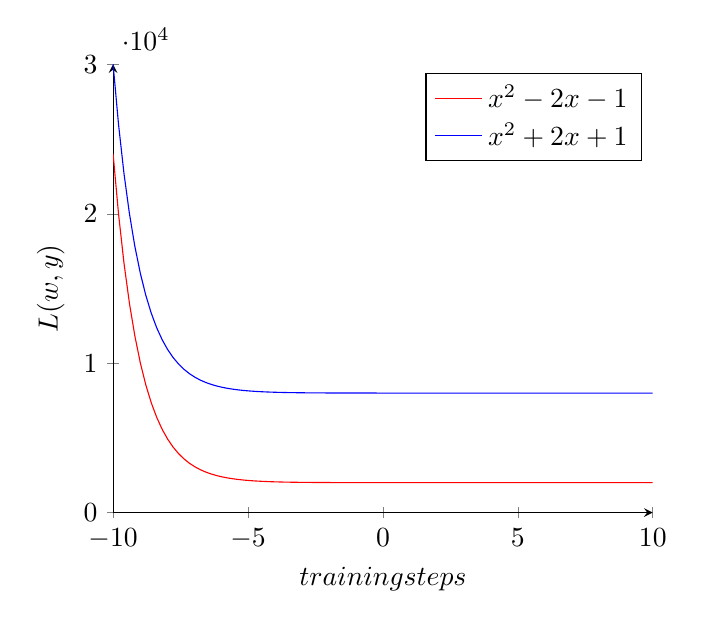
\begin{tikzpicture}
    \begin{axis}[
        axis lines = left,
        xlabel = $training steps$,
        ylabel = {$L(w,y)$},
        ymin=0,
    ]
    %Below the red parabola is defined
    \addplot [
        domain=-10:10, 
        samples=100, 
        color=red,
    ]
    {e^-x + 2000};
    \addlegendentry{$x^2 - 2x - 1$}
    %Here the blue parabloa is defined
    \addplot [
        domain=-10:10, 
        samples=100, 
        color=blue,
        ]
        {e^-x + 8000};
    \addlegendentry{$x^2 + 2x + 1$}
     
    \end{axis}
    \end{tikzpicture}
%     \caption{irgend ein plot}
%     \label{fig:ptl}
% \end{figure}

Häufig sind zu wenige Trainingsdaten oder zu komplexe/überparametrisierte
 Modelle und damit zuviele freiheitsgrade, grund für overfitting.

% hier plots von linie durch datenpunkte

% Overfitting -> hohe varianz: varianz = train_err - test_error
% Underfitting -> hoher Bias: Bias = 

Techniken um Overfitting zu vermeiden sind z.B.
\begin{itemize}
    \item Augmentierung der Daten
    \item Regularisierung der Parameter (L1/L2)
    \item Dropout
    \item early stopping
\end{itemize}

Bei Augmentierung werden aus den vorhandenen Daten künstlich mehr 
Daten generiert, in dem an den Bildern geometrische transformationen 
oder manipulationen der pixelwerte vorgenommen werden.
\\
Bei Regularisierung wird an die Lossfuction als weiterer Term
 eine aufsummierung der Gewichte gehängt, wodurch diese bei der Minimierung 
  klein gehalten werden, wodurch weniger potential zur überanpassung da ist.
  \begin{equation}
    \label{eq:regularization}
    J(w) = E + \lambda \sum_{i} w_{i}^{2}
\end{equation}

Beim Dropout werden zufällig gewichte zu 0 gesetzt.
\\
early stopping: stoppen des trainings, wenn sich overfitting einstellt.



\section{Computer Vision}

was ist Computer Vision, einordnung in ML

%---------------- SUBSECTION: Convolutional ----------------
\subsection{Convolutional Neural Networks}\label{subsec:cnn}

Für die Bilderkennung werden typischerweise Convolutionael 
Neural Networks (CNNs) verwendet. Hierbei handelt es sich um eine Erweiterung
der in \ref{sec:nn} beschriebenen Neuronalen Netze. Beim CNN 
sollen vor der Klassifikation, Merkemale des Input Bildes,
die spezifisch für eine Klasse sind herausextrahiert werden.

Dafür werden über das Bild zeilenweise Filtermatrizen mit kleinerer Dimension
(3x3, 5x5) geschoben und eine math Faltung angewendet.
Die Ergebnisse der Faltungen ergeben eine sog Feature Map, in welcher 
Muster die sowol in Filter Mtrix als auch in input Bild auftreten, verstärkt 
dargestellt werden.

Die Werte der Filter Matrizen entsprechen den zu lernenden Gewichten 
und werden mithilfe der Backpropagation angepasst.

\begin{figure}[htb]
    \centering
    \label{fig:conv}
    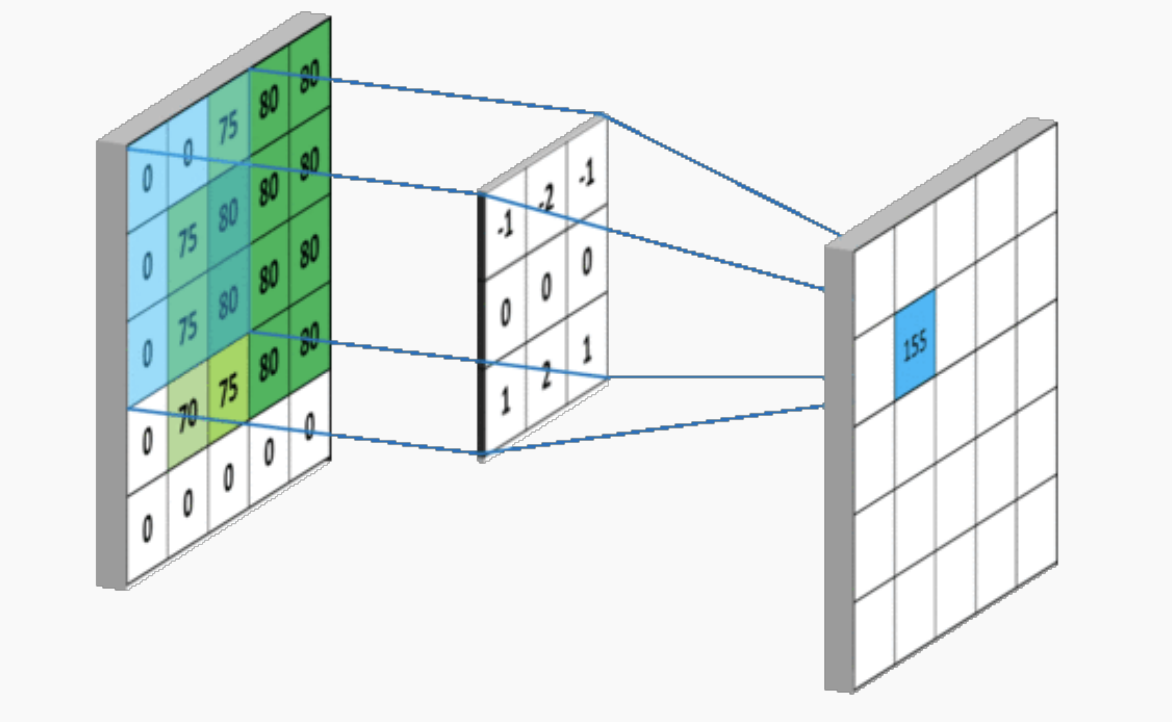
\includegraphics[width=0.4\columnwidth]{convolution.png}
    \caption{Faltung, \cite{researcherSimpleIntroductionConvolutional2019}}
\end{figure}



Durch die hintereinanderschaltung mehrerer Convolutional Layern 
lassen sich so immer komplexere Merkmale des Input Bildes in den 
Feature Maps heraus extrahieren.

Durch Subsampling Methoden wie Max Pool Layer zwischen den Convolutional
Layern verkleinert sich die Dimension der Ferture Maps in jeder Schicht.


\begin{figure}[htb]
    \centering
    \label{fig:lenet}
    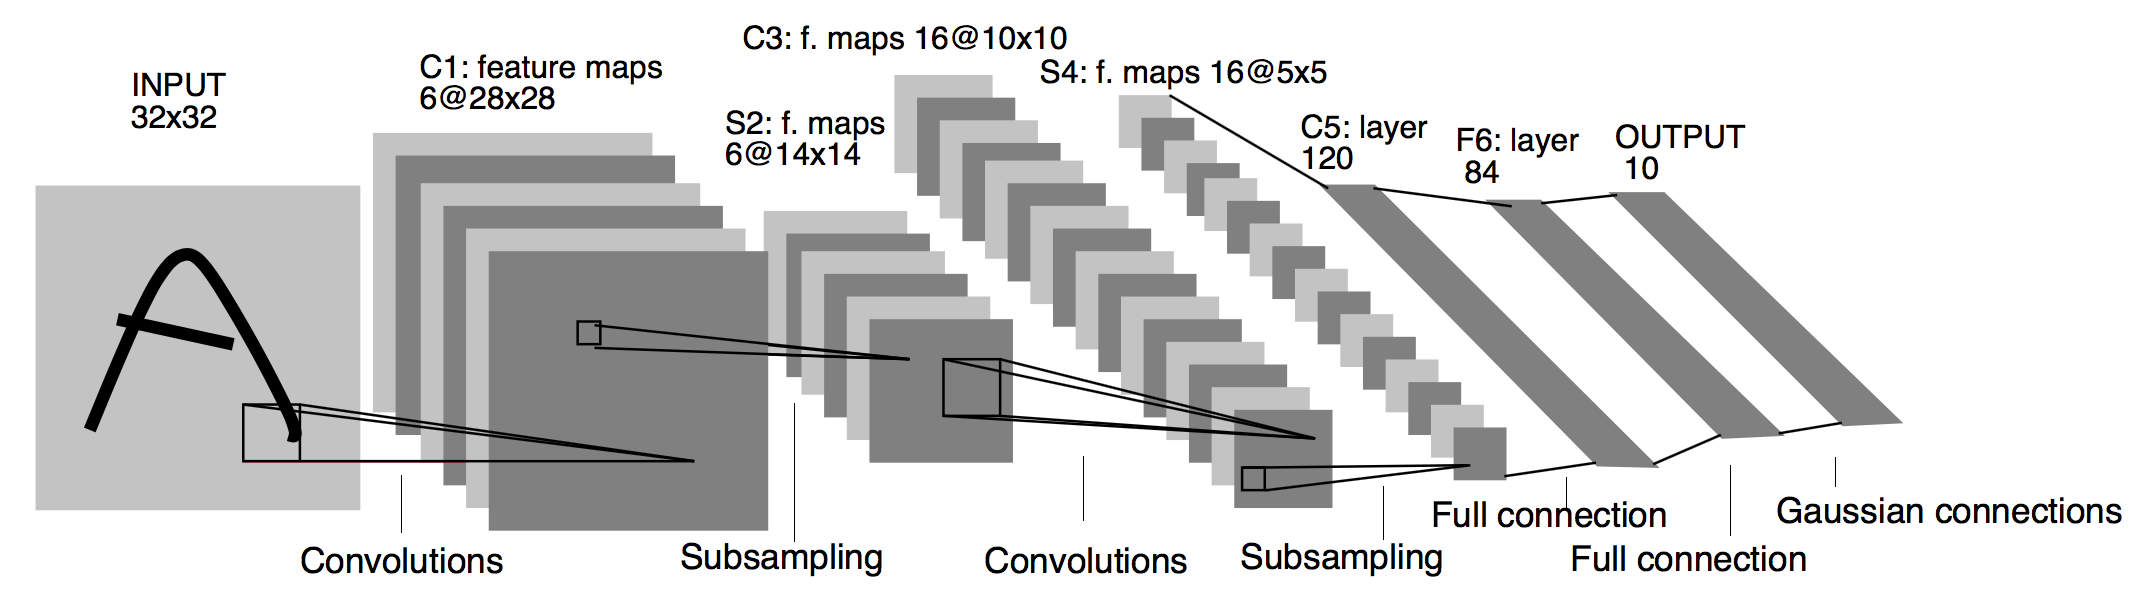
\includegraphics[width=0.8\columnwidth]{lenet.png}
    \caption{Faltung, \cite{lecunGradientBasedLearningApplied1998}}
\end{figure}


Vorteile der CNNs sind der geringere Rechenaufwand durch die gemeinsame 
Nutzung der Paramer der Filter Matrizen und die durch die 
Faltung zustande kommende räumliche invarianz für das zu erkennende 
Objekt auf dem Bild.
\\
Um die Features, welche insbesondere in den vordersten ConvLayern für 
alle klassen sehr ähnlich sind, nicht bei jedem Modell von grund auf 
neu lernen zu müssen, wird häufig \textit{Transfer Learing} angewendet, 
d.h. es werden die auf ein allg Datenset wie z.B. ImageNet vortrainierten
Gewichte verwendet und müssen so nur noch leicht für den eigenen Datensatz 
fine getuned werden.


\subsubsection{Architkturen}\label{subsubsec:architecture}

Nach der in Abbildung \ref{fig:lenet} dargestellten, erfolgreichen
ersten veröffentlichung eines CNN von YannLecunn 1998 \cite{lecunGradientBasedLearningApplied1998}
wurden wurden viele weitere Architekturen entwickelt. 

Diese werden anhand der ImageNet Chanllange ILSVRC \cite{ILSVRC15} bewerted

Die bekanntesten gewinner Modelle sind wie in \cite{StanfordCS231nConvolutional}
aufgeführt:


\begin{itemize}
    \item Alexnet (2012), mehrere conv layer hintereinander
    \item GoogleLeNet (2014), Inception Module
    \item VGGNet 2014
    \item ResNet (2015), 
\end{itemize}

%---------------- SUBSECTION: Obj Detection ----------------
\subsection{Objekt erkennung}\label{subsec:objdet_det}

Neben der Information, was sich auf einem Bild befindet möchte
man bei der Object Detection auch herausfinden wo sich das 
Objekt befindet.
Dafür wird ein in \ref{subsec:cnn} beschriebenes CNN als Basis 
zusammen mit weiteren Mechanaismen, auf die in \ref{sec:related_work}
genauer eingegangen wird, verwendet.
\begin{figure}[htb]
    \centering
    \label{fig:class_vs_det}
    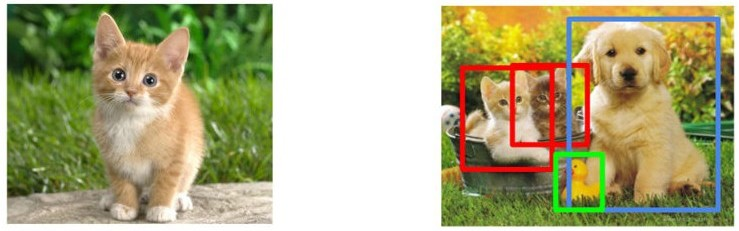
\includegraphics[width=0.8\textwidth]{classification_detection_small.jpeg}
    \caption{Unterschied: Classification - Detection}
\end{figure}


%------------------- SUBSECTION: ML Frameworks ---------------
\subsection{Deep Learing Lerining Frameworks}
kurz Frameworks all.\\
dann speziell tensorflow (kein obj det api)



%------------------- SECTION: Hardware ----------------------
\section{Hardware/NCS2}\label{sec:hardware}
%noch eine section zu Hardware allg (cpu, gpu, tpu), Neural Compute Stick und AI on the egde

Da das Training und die Inferenz von Deep Learning Algorithmen
 sehr rechenintensiv ist, werden entsprechen leistungsfähige 
Prozessoren benötigt. Dabei ist die Ausführung auf einer GPU 
(Graphical Processor Unit) meist effizienter als auf einer 
CPU (Central Processor Unit). Anwendungen auf eingebetteten Systemen
wie z.B. einplatinen Computern wie dem in der Arbeite verwendeten
Raspberry Pi kommen dabei schnell an ihre Grenzen.
Möchte man dennoch die Daten auf dem Gerät verrechnen und 
nicht an eine Cloud senden, bieten verschiedene KI Beschleuniger 
die möglichketi die Inferenz des Deep Learning Modells 
auf externer Hardware auszuführen. Einer davon ist der in der 
Arbeit verwendete Neural Compute Stick 2 von Intel.
\\
Dieser basiert auf der Movidius Myriad X Vision Processing Unit (VPU)
\cite{haussermannFunktionUndEffizienz}

\begin{figure}[htb]
    \centering
    \label{fig:ncs2}
    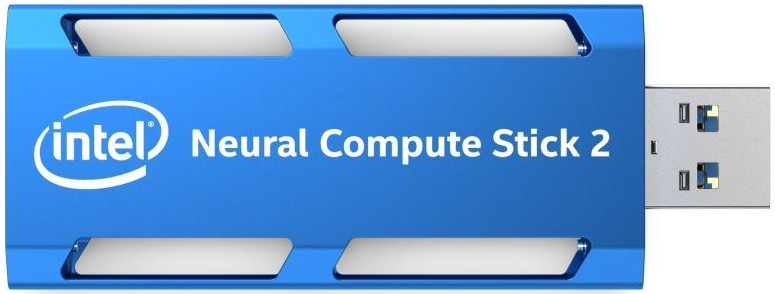
\includegraphics[width=0.4\columnwidth]{ncs2_top.jpg}
    \caption{NCS2}
\end{figure}

\subsection{OpenVino Toolkit}

% überlegung: hier auch noch restl. hardware erläutern: raspi, cam, internet

\begin{itemize}
    \item 
\end{itemize}